\section{CALoE library}

In this section, we explain the main features of the CALoE library including data types and functions.

\subsection{Basic concepts}

CALoE library is divided into two different layers (high level and low level). Additionally, some example code is provided with the library.

\begin{figure}[H]
\centering
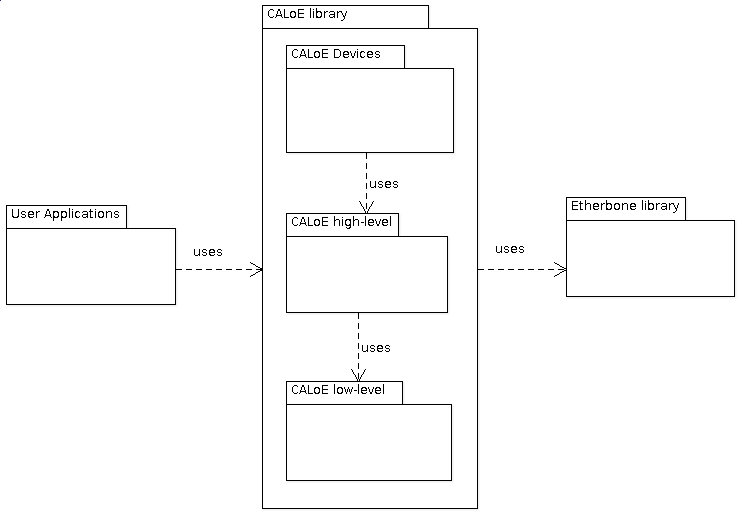
\includegraphics[width=350px,height=300px]{img/PackageDiagram.png}
\caption{CALoE Package Diagram}
\label{caloe_pd_img}
\end{figure}

In Figure \ref{caloe_pd_img}, you can see the Package Diagram with the main design layers of CALoE. It contains two main layers: high level and low level layer.
The first one implements all classes to manage access and all additional structures as a hash map for each device.The second one tries to hide Etherbone library
implementation details for the high level layer. It implements the low level necessary access and structures to perform these actions with the Etherbone library methods.

\begin{figure}[H]
\centering
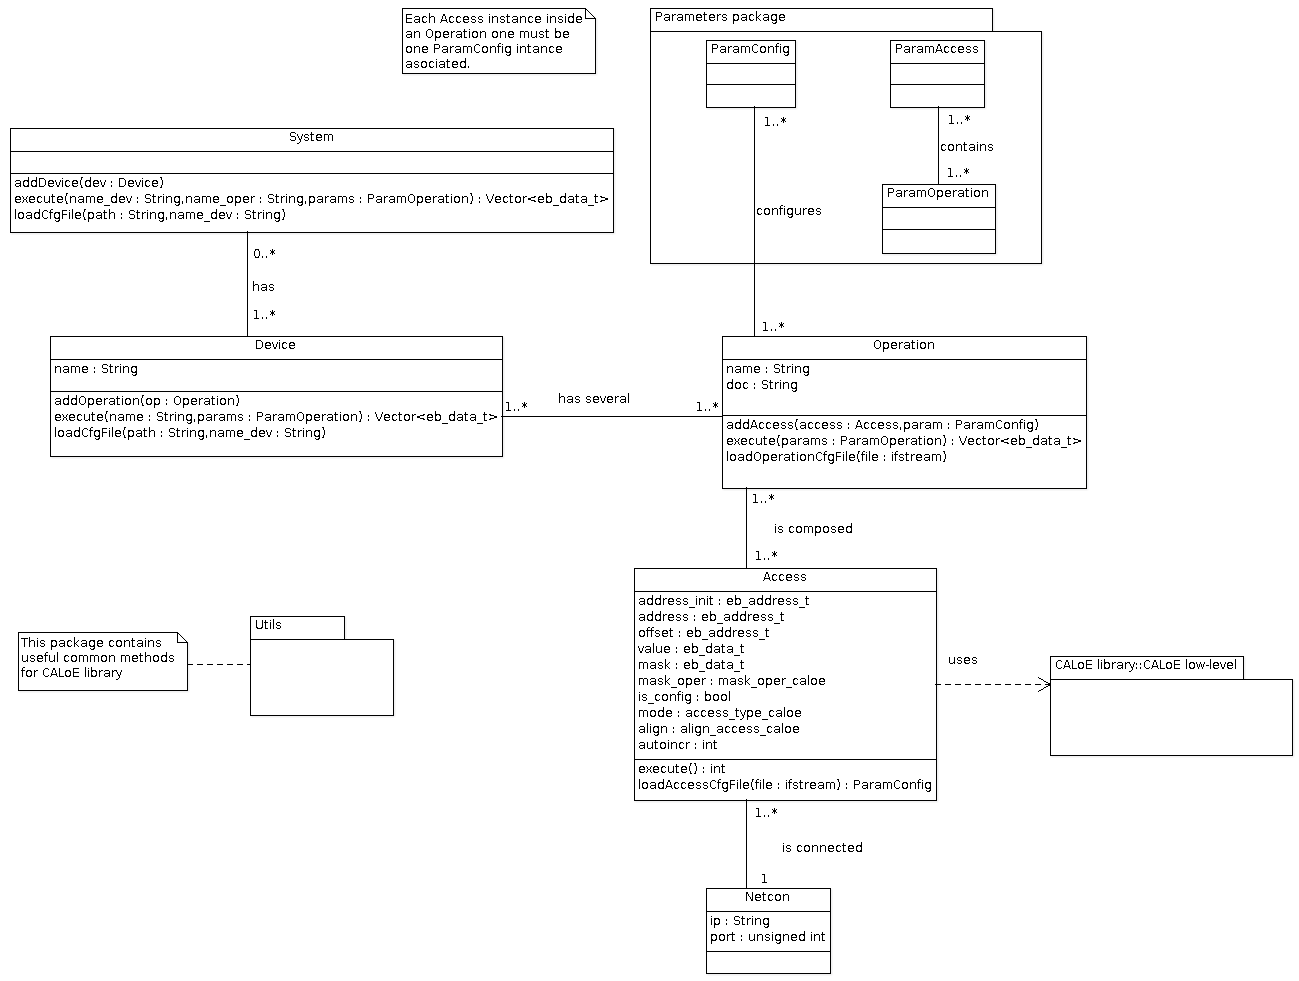
\includegraphics[width=450px,height=400px]{img/high_level_class_diagram.png}
\caption{CALoE high level layer class diagram}
\label{caloe_hl_cd_img}
\end{figure}

Figure \ref{caloe_hl_cd_img} describes the high level layer class diagram of CALoE. It contains all structures
to store the device table (inside the System class) and operation table (inside the Device class) for each device. Each operation contains
a list of necessary accesses and for each access, network parameters (as IP address and port) must be given. 
It is worth mentioning that another package exists in this level. Parameters package
contains classes to store needed parameters for accesses. ParamConfig class is a specification of formal parameters and 
ParamAccess class contains current values of them. ParamOperation contains a list of ParamAccess to perform an operation.

\begin{figure}[H]
\centering
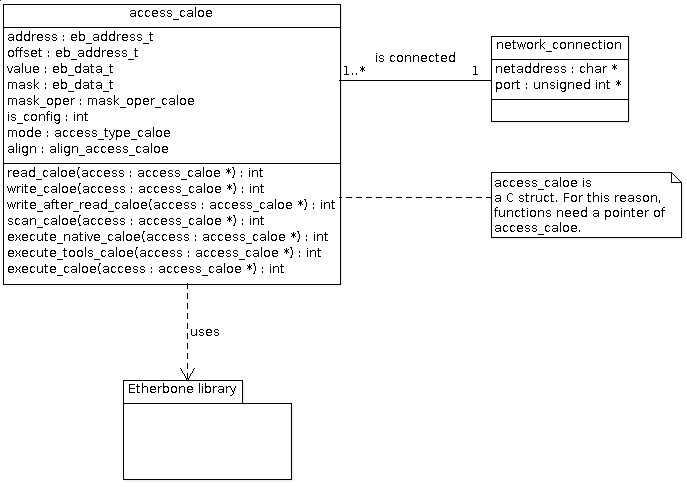
\includegraphics[width=300px,height=250px]{img/low_level_class_diagram.png}
\caption{CALoE low level layer class diagram}
\label{caloe_ll_cd_img}
\end{figure}

Low level data structures are shown in Fig \ref{caloe_ll_cd_img}.

\subsubsection{Access}

CALoE is based on an access concept. An access is a basic operation (read, write, write after read and scan) that can be performed in a device. Basically, we can define four different access methods:

\begin{itemize}
 \item {\textbf{Read} retrieves data from device address. }
 \item{\textbf{Write} changes content of one memory position of a device. }
 \item{\textbf{Write after read} is a special kind of write, it reads value from one memory position and modifies one part of its content (it filters the received data with a predefined bit-mask). \textbf{Write after read} is very useful when you want to write only a part of word but not the entire word (it saves a part of the previous content). }
 \item{\textbf{Scan} can get the SDB structure of device. It is very useful to know the device memory map.}
\end{itemize}

Access is implemented in both low and high level layers of CALoE. 

Low level layer defines access in access\_internals source file in which you can find network primitives with Etherbone API. 
access\_internals source file defines the following:

\begin{itemize}
\item{\textbf{network\_connection:} contains network connection information of devices such as IP netaddress and port number.}
\item{\textbf{access\_caloe:} main action in CALoE library. It can be write, read, write after read or scan.}
\begin{itemize}
\item{\textbf{address:} access memory address.}
\item{\textbf{offset:} it will be added to the memory address before the access is executed.}
\item{\textbf{value:} value to be written or returned value of access.}
\item{\textbf{mask:} it will be applied to value before writting it or will be applied to value after reading it.}
\item{\textbf{mask\_oper:} indicates if an OR or AND mask operation must be applied.}
\item{\textbf{is\_config:} indicates if the memory address is refered to the Etherbone configuration space or not.}
\item{\textbf{mode:} access type (READ, WRITE, READ\_WRITE, SCAN).}
\item{\textbf{align:} access word size (1 byte, 2 bytes, 4 bytes or 8 bytes).}
\item{\textbf{networkc:} contains IP address and port.}
\end{itemize}
\end{itemize}

Included functions in low level layer are:

\begin{itemize}
\item{\textbf{read\_caloe:} implements read access with Etherbone primitives.}
\item{\textbf{write\_caloe:} implements write access with Etherbone primitives.}
\item{\textbf{write\_after\_read\_caloe:} implements write after read using read\_caloe and write\_caloe functions.}
\item{\textbf{scan\_caloe:} implements scan access with Etherbone primitives.}
\item{\textbf{execute\_tools\_caloe:} it calls eb-ls, eb-read or eb-write Etherbone command depending of access type.}
\item{\textbf{execute\_native\_caloe:} it calls read, write, write after read or scan primitive function depending of access type.}
\item{\textbf{execute\_caloe:} it calls execute\_tools\_caloe or execute\_native\_caloe depending of CALOE\_MODE flag.}
\end{itemize}

The above functions are based on eb-ls, eb-write, eb-read tools of Etherbone project \cite{Etherbone-repo}.

High level layer implements a wrapper in Access class. Main Access methods are:

\begin{itemize}
\item{\textbf{loadCfgFile:} loads an access configuration file into class fields.}
\item{\textbf{execute:} executes one access. This method calls low level access functions.}
\end{itemize}

For further details, please see doxygen project documentation (in doxygen folder).

\subsubsection{Parameters}

Parameter classes have two goals:

\begin{itemize}
 \item {Specify what is needed by an access (ParamConfig class).}
 \item {Store user parameters for an operation (ParamOperation and ParamAccess classes).}
\end{itemize}

Methods in Parameter classes are very simple and, for this reason, we do not describe here.

For further details, please see doxygen project documentation (in doxygen folder).

\subsubsection{Operation}

Operation is a structure that stores several accesses (in a sequential container). Each operation includes a unique name and an optional description. 
When you execute an operation, all its accesses are filled in with user arguments. This action is performed sequentially. 

Main methods in Operation class are:

\begin{itemize}
\item{\textbf{loadCfgFile:} loads a device configuration file and adds a new Device instance in System.}
\item{\textbf{execute:} executes one operation of one device in your System. It searches this Device and call its execute method.}
\item{\textbf{addAccess:} adds new Access and ParamConfig instances to Operation.}
\end{itemize}

For further details, please see doxygen project documentation (in doxygen folder).

\subsubsection{Device}

Device is a structure that stores several operations using a hash table. User can initialize devices loading configuration files. Then, user can execute a device operation with its name.

The Device class has several methods but the most relevant ones are:

\begin{itemize}
\item{\textbf{loadCfgFile:} loads a device configuration file and adds a new Device instance in System.}
\item{\textbf{execute:} executes one operation of one device in your System. It searches this Device and call its execute method.}
\item{\textbf{addOperation:} adds new Operation to Device.}
\end{itemize}

For further details, please see doxygen project documentation (in doxygen folder).

\subsubsection{System}

System contains several devices that can be referenced by their names. System is used when user wants to define an entire system with multiple devices.

The most important system methods are:

\begin{itemize}
\item{\textbf{loadCfgFile:} loads a device configuration file and fills Access instance in. it also returns a ParamConfig instance for this Access.}
\item{\textbf{execute:} executes this access using low-level layer methods.}
\item{\textbf{addDevice:} adds a new Device to System.}
\end{itemize}

For further details, please see doxygen project documentation.

\subsection{Example of CALoE API}

\definecolor{mygreen}{rgb}{0,0.6,0}
\definecolor{mygray}{rgb}{0.5,0.5,0.5}
\definecolor{mymauve}{rgb}{0.58,0,0.82}

\lstset{ %
  backgroundcolor=\color{white},   % choose the background color; you must add \usepackage{color} or \usepackage{xcolor}
  basicstyle=\footnotesize,        % the size of the fonts that are used for the code
  breakatwhitespace=false,         % sets if automatic breaks should only happen at whitespace
  breaklines=true,                 % sets automatic line breaking
  captionpos=b,                    % sets the caption-position to bottom
  commentstyle=\color{mygreen},    % comment style
  extendedchars=true,              % lets you use non-ASCII characters; for 8-bits encodings only, does not work with UTF-8
  frame=single,                    % adds a frame around the code
  keepspaces=true,                 % keeps spaces in text, useful for keeping indentation of code (possibly needs columns=flexible)
  keywordstyle=\color{blue},       % keyword style
  language=C++,                 % the language of the code
  numbers=left,                    % where to put the line-numbers; possible values are (none, left, right)
  numbersep=5pt,                   % how far the line-numbers are from the code
  numberstyle=\tiny\color{mygray}, % the style that is used for the line-numbers
  rulecolor=\color{black},         % if not set, the frame-color may be changed on line-breaks within not-black text (e.g. comments (green here))
  showspaces=false,                % show spaces everywhere adding particular underscores; it overrides 'showstringspaces'
  showstringspaces=false,          % underline spaces within strings only
  showtabs=false,                  % show tabs within strings adding particular underscores
  stepnumber=1,                    % the step between two line-numbers. If it's 1, each line will be numbered
  stringstyle=\color{mymauve},     % string literal style
  tabsize=2,                       % sets default tabsize to 2 spaces
  title=\lstname                   % show the filename of files included with \lstinputlisting; also try caption instead of title
}

\begin{lstlisting}[frame=single, label=config_file_example1a, caption=Example of CALoE API]
System sys;

vector<eb_data_t> res;

ParamOperation params_dio;
ParamOperation params_vuart;
ParamAccess param;

String ip("udp/192.168.10.90");
int ch = 0;

// Add two devices into System
sys.loadCfgFile("dio.cfg","dio");
sys.loadCfgFile("vuart.cfg","vuart");
	
// Set IP and mask as parameters.
param.setIP(ip);
param.setMask(ch);

params_dio.addParameter(param);
params_dio.addParameter(param);
params_dio.addParameter(param);

// Configure channel as Output
sys.execute("dio","config_channel_O",params_dio);
\end{lstlisting}

\begin{lstlisting}[frame=single, label=config_file_example1b, caption=Example of CALoE API (cont)]
// Reset ParamAccess
param.reset();

// Set IP
param.setIP(ip);

params_vuart.addParameter(param);

// Execute vuart_ready

res = sys.execute("vuart","vuart_ready",params_vuart);
	 
int data = res.at(0);

if (data == 0) {
	cout <<"Vuart is ready to write"<<endl;
}
else {
	cout <<"Vuart is busy"<<endl;
}
\end{lstlisting}

\subsection{Configuration files}

CALoE library allows the user to define their own configuration files.

\lstset{language=Bash,
 morekeywords={EOPERATION, BOPERATION, EACTION, BACTION, NET, NETP, MODE, ADDRESS, NAME, DOC, ALIGN, MASK, OFFSET, MSKPOS, MSKNEG, AUTO, VALUE, VALUEP, PORT, PORTP}}

\begin{lstlisting}[frame=single, label=config_file_example1, caption=Example of configuration file]
# vuart_read operation: it reads one character from uart
BOPERATION
	NAME vuart_read
	DOC Read a value from vuart

	BACTION
		NETP
		ADDRESS 0x20514
		MODE R
		ALIGN 4
	EACTION

EOPERATION
\end{lstlisting}

We explain in detail the necessary sintax to perform it.

\begin{itemize}
 \item {You can put comments with \# at the begining of a line.}
 \item {One operation begins with the BOPERATION token and ends with the EOPERATION one. Inside one operation, you must set a name using NAME token. Additionally, put DOC token if you want to specify a brief description.}
 \item{As seen in previous sections, one operation contains several accesses. Each access begins with the BACTION token and ends with the EACTION one. Inside one access/action you must indicate all needed fields or mark them as parameters.}
 \begin{itemize}
    \item{To specify netaddress, NET or NETP tokens must be used. Former is following by netaddress value like udp/<ip>. Latter marks netaddress like parameter.}
    \item{Port and Value can be filled in the same way than netaddress. Use PORT or PORTP for port and VALUE and VALUEP for value. Note 'P' indicates parameter like netaddress case.}
    \item{Address must be fixed in configuration file. So, you only can put ADDRESS token and then, a number contains access's address. Similarly, align and mode must be fixed in the same way than address. Use ALIGN and MODE respectively for this.}
    \item{If you want to access to contiguous addresses, you can use autoincrement/decrement mode. You can use  AUTO <N> in order to perform this type of access.}
    \item{Finally, you can specify mask and offset attributes. Offset is always one parameter and its syntax is OFFSET \{offset1,offset2,...,offsetN\}. Mask can be parameter or fixed value. If you want to use it as fixed value, you must put MASK <value> and you can specify mask operation with MSKPOS (OR) or MSKNEG (AND). If you want to use it as parameter, syntax is MASKP \{mask1,mask2,...,maskN\}. Remember, in main program, you must indicates index of vector for OFFSET and MASK param (index begins in 0).}
 \end{itemize}
\end{itemize}

If you need more information, you can consult devices/Dio/dio.cfg or device/Vuart/vuart.cfg file.

\subsection{Supported devices}

In this section, we explain two configuration files developed as an example of how to build simple command operations over CALoE library easily. 
The folowing example is based on SPEC \cite{Spec-board} + DIO-FMC card \cite{dio-fmc-repo}, WR NIC \cite{WR-nic} project gateware and WRPC software \cite{WRPCSW-repo}.
Starting kit project \cite{WR-starting-kit} helps to build WR-NIC gateware and sotfware. 

\begin{figure}[H]
\centering
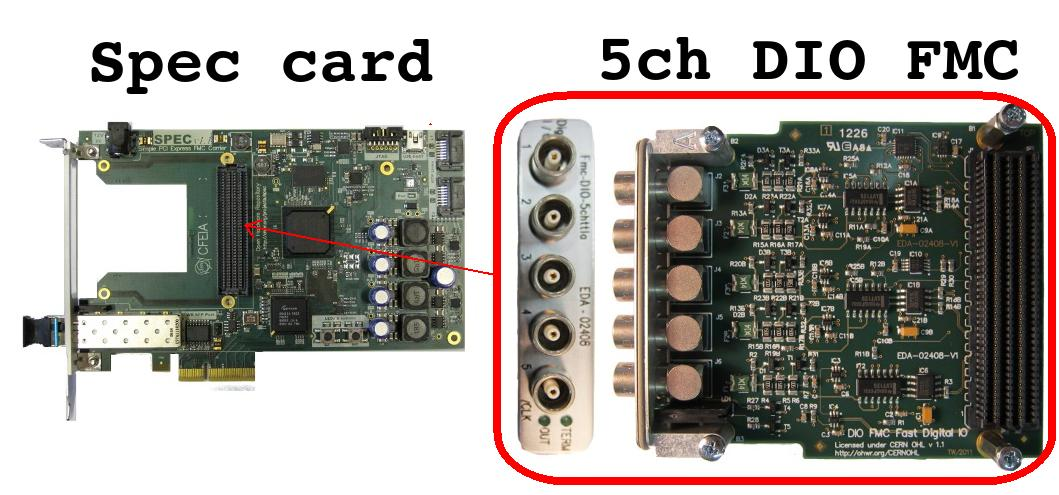
\includegraphics[width=400px,height=200px]{img/spec_dio.jpg}
\caption{SPEC + 5ch DIO FMC card}
\label{spec_dio_fmc_img}
\end{figure}

CALoE library supports the following devices:

\begin{itemize}
 \item {\textbf{Dio:} This class loads DIO-FMC configuration file and allows to manage this device. The main implemented operation are:}
 \begin{itemize}
      \item{Generate an immediate pulse.}
      \item{Generate a programmable time pulse.}
      \item{Configure a card channel as Input/Output with/without resistor termination.}
      \item{Get FIFO timestamps from one/all channel/s.}
      \item{Check if one channel FIFO is empty/full and how many timestamps it has.}
 \end{itemize}
 \item {\textbf{Vuart:} This class loads Vuart configuration file and allows to send commands to the LM32 procesor in WRPC as it would be connected by USB port (it emulates the operation of spec-vuart in spec-sw repository \cite{SPECSW-repo}).}
\end{itemize}

\begin{figure}[H]
\centering
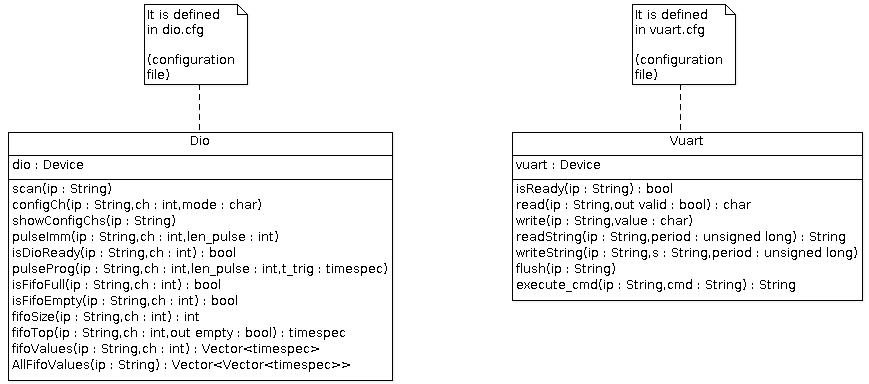
\includegraphics[width=400px,height=200px]{img/caloe_devices.png}
\caption{Supported devices class diagram}
\label{supported_dev_cd_img}
\end{figure}

The figure \ref{supported_dev_cd_img} describes device classes developed and their operations.

You can get more information about these devices in devices folder of CALoE project.

\subsection{Tools}

We have developed a tool in order to test all functionalities offered by the CALoE library that includes examples for the supported devices. This tool source code is also available in tools folder.

\subsubsection{cmd\_spec tool}

\textbf{cmd\_spec} allows you to control one SPEC card remotely. It shows a prompt in which you can write command to be executed by SPEC card.

\begin{figure}[H]
\centering
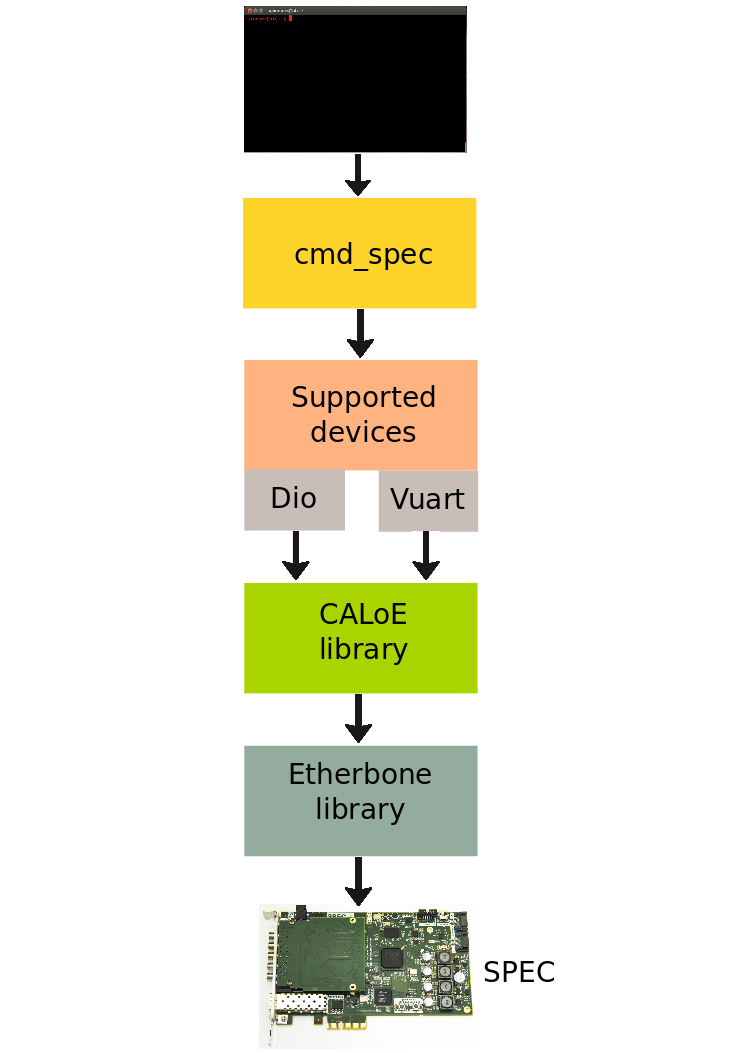
\includegraphics[width=200px,height=300px]{img/cmd_spec.png}
\caption{cmd\_spec overview}
\label{cmd_spec_overview_img}
\end{figure}

All available commands are:

\begin{itemize}
 \item {\textbf{fifo\_val: }Show timestamps of one channel.}
 \item {\textbf{all\_fifo\_val: }Show timestamps of all channels.}
 \item {\textbf{scan: }Get SDB information of device.}
 \item {\textbf{pulse\_imm: }Generate an immediate pulse.}
 \item {\textbf{pulse\_prog: }Generate a programmable time pulse.}
 \item {\textbf{config\_ch: }Configure one channel as Input/Output with/without resistor termination.}
 \item {\textbf{show\_config\_ch: }Show configuration of all channels.}
 \item {\textbf{fifo\_empty: }Check if channel FIFO is empty.}
 \item {\textbf{fifo\_full: }Check if channel FIFO is full.}
 \item {\textbf{fifo\_size: }Get number of timestamps of one channel FIFO.}
 \item {\textbf{vuart: }Change to Vuart mode in order to send commands to the LM32 in WRPC.}
\end{itemize}

Following figures show some use cases of cmd\_spec tool.

\begin{figure}[H]
\centering
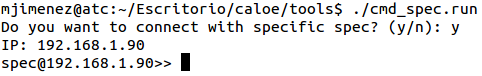
\includegraphics[width=400px,height=75px]{img/cmd_spec_prompt.png}
\caption{cmd spec prompt}
\label{cmd_spec_prompt_img}
\end{figure}

\begin{figure}[H]
\centering
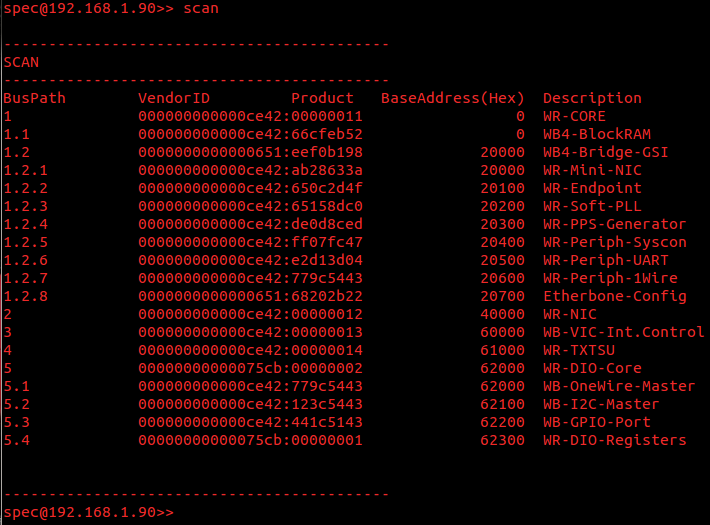
\includegraphics[width=500px,height=400px]{img/cmd_spec_scan_sdb.png}
\caption{cmd spec sdb scan operation}
\label{cmd_spec_scan_img}
\end{figure}

\begin{figure}[H]
\centering
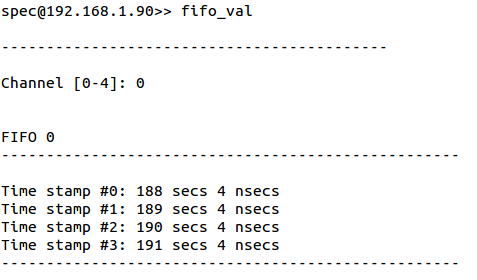
\includegraphics[width=400px,height=400px]{img/cmd_spec_dio_fifo.png}
\caption{cmd spec fifo val operation}
\label{cmd_spec_fifo_val_img}
\end{figure}

\begin{figure}[H]
\centering
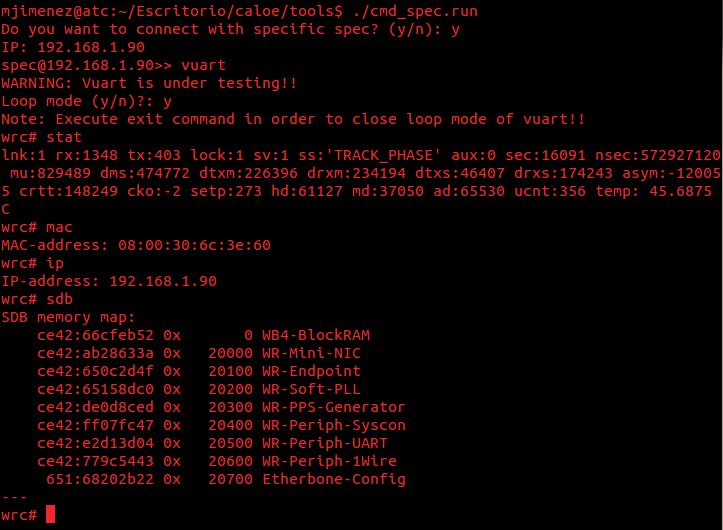
\includegraphics[width=500px,height=400px]{img/cmd_spec_vuart.png}
\caption{cmd spec vuart operation}
\label{cmd_spec_vuart_img}
\end{figure}

\subsection{Compilation}

In order to compile the CALoE library and any of the applications it uses, we have written a Makefile file to simplify process.

You must only run the following commands:

\lstset{language=Bash}

\begin{lstlisting}[frame=single, label=make_caloe, caption=Compiling CALoE library\, devices and tools]
cd <CALoE main dir>
make
\end{lstlisting}

If you want to generate doxygen documentation of source code, you must execute:

\begin{lstlisting}[frame=single, label=make_doxygen, caption=Compiling CALoE library doxygen documentation]
cd <CALoE main dir>
make build-doxygen
\end{lstlisting}

Finally, If you want to generate this document, you must execute:

\begin{lstlisting}[frame=single, label=make_doc, caption=Compiling CALoE library documentation]
cd <CALoE main dir>
make build-doc
\end{lstlisting}
